\chapter{対話型遺伝的アルゴリズム}
本章では,本システムで使用した対話型遺伝的アルゴリズムを概説する.

\section{遺伝的アルゴリズム}
遺伝的アルゴリズム(Genetic Algorithm; GA)は生物が環境に適応し進化する過程を模倣した最適解探索アルゴリズムであり,1975年にJohn Holandら
\cite{Holland75}によって提案された.
問題に対する解を染色体で表現し,解としての良さを適応度として,複数個体の中から適応度が高い個体の形質が継承されるように,選択,交叉,突然変異により次世代の個体集団を生成する.
世代交代を繰り返し行い,適応度の高い個体を探索する.
終了条件には,世代交代数や適応度に対する閾値の設定などがある.
終了条件を満たしたら,最終世代の最良個体を出力して処理を終了する.
GAの処理手順を図\ref{ga_proces}に示す.

\begin{figure}[b!]
    \begin{center}
    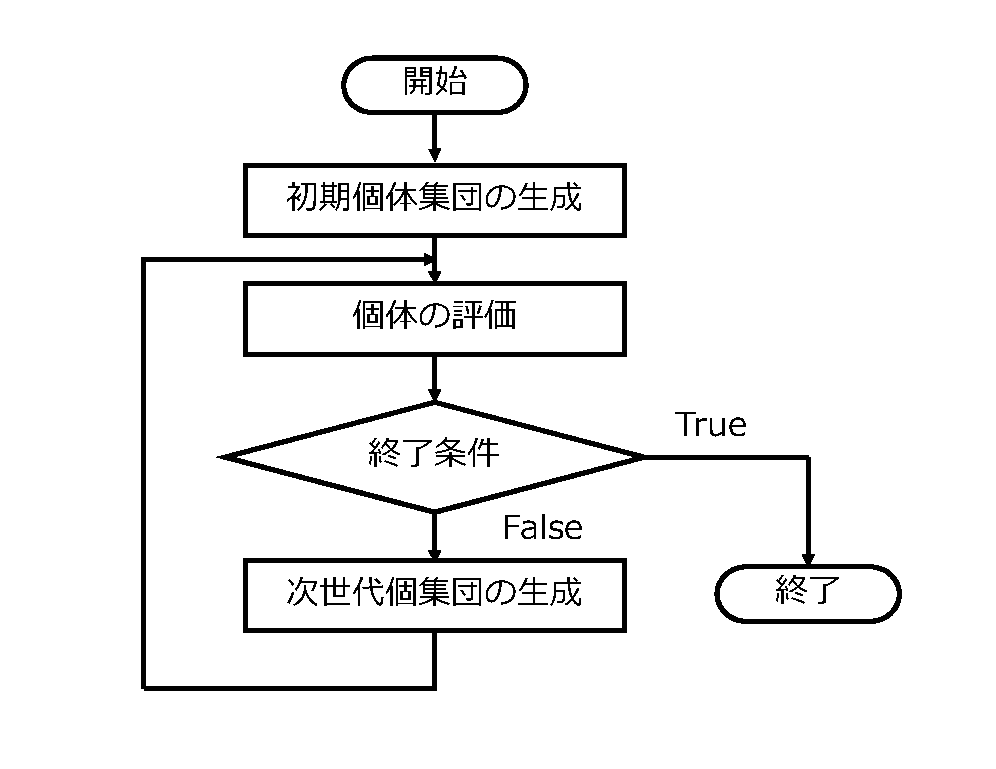
\includegraphics[scale=0.62]{image/ga_proces.eps}
    \caption{GAの処理手順}
    \label{ga_proces}
    \end{center}
\end{figure}

% \section{対話型遺伝的アルゴリズム}
% 対話型遺伝的アルゴリズム(Interactive Genetic Algorithm; IGA)とは,GAの処理の一部である適応度関数での個体の評価を人間が行い,解を探索する方法である.
% 適応度関数の設定が困難な楽曲生成や,画像生成などの個人の感性によって評価が異なる問題に用いられる.
% 人間が個体を評価するため,個人の好みを個体に反映させることができる.
% しかし,人間がすべての評価を行うため負担が大きくなる問題がある.
% したがって,世代交代数と個体数を一般的なGAよりも少なくする必要がある.
% また,世代交代数が少ないため,突然変異が起こりにくくなる.
% したがって,GAよりも突然変異率が大きく設定される.

\subsection{染色体表現}
生物の形質は染色体に含まれている遺伝子によって決定される.
GAでは,染色体は解候補,遺伝子は解の構成要素を表現している.
遺伝子は,一般的に数値やビット列などを用いて表現される.
遺伝子の染色体上での位置を遺伝子座,染色体として表される遺伝子の構成を遺伝子型,遺伝子を問題に対応する形式に変換したものを表現型,遺伝子がとりうる値を対立遺伝子と呼ぶ.
染色体の例を図\ref{ga_chrom}に示す.

\begin{figure}[t]
    \begin{center}
    \includegraphics[scale=0.6]{image/ga_chrom.eps}
    \caption{染色体の例}
    \label{ga_chrom}
    \end{center}
\end{figure}

\subsection{親個体の選択}
GAでは,親個体の形質を受け継いで次世代の子個体を生成する.
環境に適応した生物ほど子孫を残すように,適応度が高い個体ほど親に選ばれる確率を高くする.
親個体を選択する方法には,ルーレット選択,ランキング選択,トーナメント選択などが存在し,それぞれ特徴がある.

\subsubsection{ルーレット選択}
ルーレット選択は,各個体の適応度に比率を選択確率の比率にする方法である.
一般的なルーレットの円盤は各領域が均等に割り当てられているが,ルーレット選択では領域が不均等に分けられている円盤を用いる.
面積の比が各個体の適応度の比になるように各個体に対応する領域に分ける.
円盤上の一点をランダムに選び,選ばれた点の領域に対応する個体を親個体とする.
円盤全体の面積に対する各個体に対応する領域の面積の割合が各個体が選択される確率に相当する.
したがって,個体$I_k$の適応度が$fitness$(${ I_k}$)のとき,ルーレット選択によって選択される確率$rouProb$(${I_k}$)は,式\ref{eq0301}で求められる.

    \begin{equation}\label{eq0301}
        {rouProb}({I_k}) = \frac{{fitness}({I_k})} {\displaystyle\sum_i{{fitness}({I_i})}}
    \end{equation}
分母はすべての個体の適応度の和である.
ルーレット選択では,適応度の比率で選択確率を決めるため,適応度が一様になると選択確率も一様になる問題がある.
例として,適応度が150の個体A,適応度が30の個体B,適応度が25の個体C,適応度が22の個体Dのルーレットを図\ref{ga_roulette}に示す.
適応度が最も大きい個体Aが最も選択される確率が高い.
しかし個体B,C,Dは適応度の差が小さいため,各個体が選択される確率は一様である.

\begin{figure}[t]
    \begin{center}
    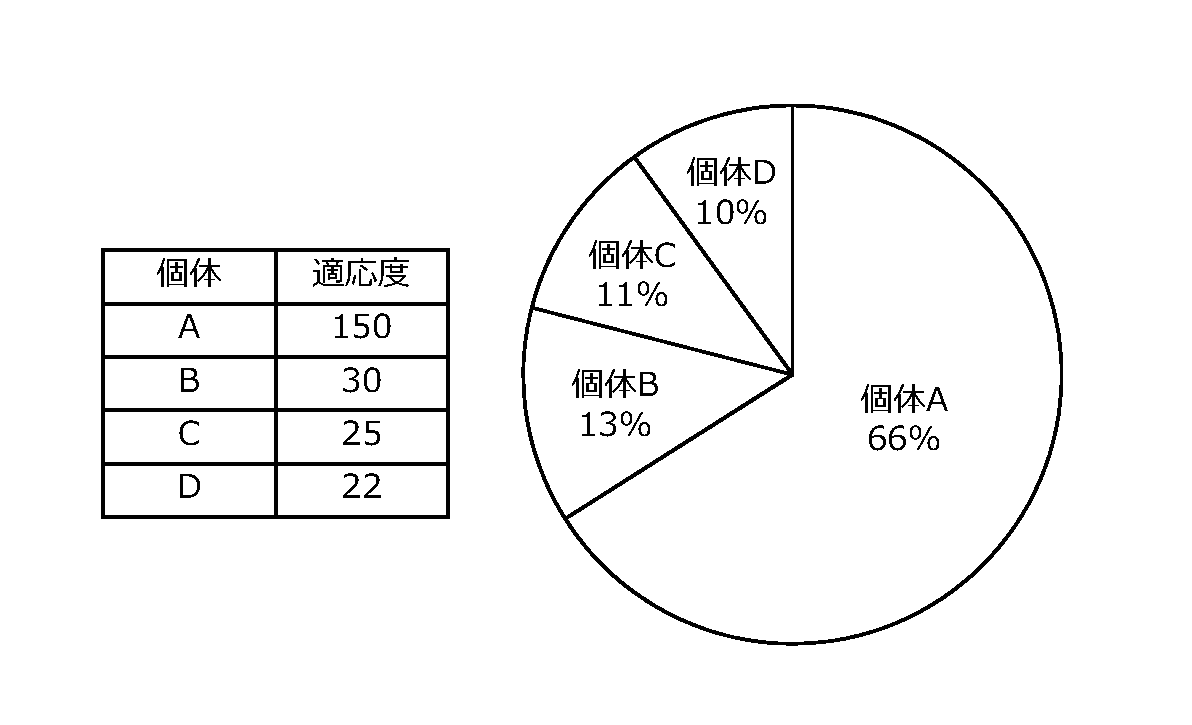
\includegraphics[scale=0.5]{image/ga_roulette.eps}
    \caption{ルーレット選択}
    \label{ga_roulette}
    \end{center}
\end{figure}



\subsubsection{トーナメント選択}
トーナメント選択は,個体集団内からの$S$個の個体をランダムに抽出し,最も適応度の高い個体を選択する.
$S$の値を調整することで,目的に合わせて適応度の低い個体が選択される確率を調整することが可能である.
$S$が大きいほど,適応度の低い個体は選択されにくくなる.
トーナメント選択の例を図\ref{ga_tournament}を示す.

\begin{figure}[b!]
    \begin{center}
    \includegraphics[scale=0.55]{image/ga_tournament.eps}
    \caption{トーナメント選択}
    \label{ga_tournament}
    \end{center}
\end{figure}

\subsubsection{ランキング選択}
ランキング選択は,個体の適応度をもとに各個体の順位を決め,各順位に応じた選択確率によって親個体を選択する手法である.
個体$I_k$の順位が${rank(I_k)}$のとき,選択される確率$ranProb$(${I_k}$)は,式\ref{eq0302}で求められる.

    \begin{equation}\label{eq0302}
        {\it ranProb}({\it I_k}) = \frac{{\it M} - {\it rank}({\it I_k}) + 1} {\displaystyle\sum_i{{\it rank}({\it I_i})}} = \frac{{\it M} - {\it rank}({\it I_k}) + 1}{\frac{1}{2}{\it M}({\it M}+1)}
    \end{equation}
式において,$M$は個体集団の個体数である.
ランキング選択では,適応度の差は反映せず,各個体の順位のみで選択確率が決まる.
表\ref{rank}の例では,個体Aと個体Cの適応度の差は200,個体Dと個体Bの差は2だが,それぞれの個体間の選択確率の差はいずれも10\%になる.
したがって,適応度に大きな差があっても順位が近ければ,優良個体と近い選択確率になる.また,適応度に差がなくても選択確率が大きく変わる可能性がある.
一方,順位で選択確率を決めるため,ルーレット選択でみられる選択確率が一様になる問題を回避できる.

\begin{table}[t]
	\centering
	\caption{ランキング選択における選択確率の例}
	\begin{tabular}{|c|c|c|c|} \hline
	順位   & 個体名 & 適応度 & 選択確率 \\ \hline
	1      & A & 250 & 40\% \\ \hline
	2      & C & 50 & 30\% \\ \hline
	3      & D & 20 & 20\% \\ \hline 
	4      & B & 18 & 10\% \\ \hline 
	\end{tabular}
	\label{rank}
\end{table}



\subsection{交叉}
交叉とは,選択により選ばれた2つの親個体間で遺伝子を交換することで,新たな子個体を生成する処理である.
交叉には,一点交叉,多点交叉,一様交叉などの手法がある.
一点交叉は交叉点をランダムで一か所選び,その前後で遺伝子を交換する手法である.
多点交叉では,交叉点をランダムで複数選び,区切られた交叉点間で遺伝子を交換する.
一様交叉では,遺伝子座ごとにどちらの親の遺伝子を受け継ぐかを独立して決める.
各交叉の例を図\ref{ga_cross}に示す.

\begin{figure}[htbp]
    \begin{center}
    \includegraphics[scale=0.6]{image/ga_cross.eps}
    \caption{各交叉の例}
    \label{ga_cross}
    \end{center}
\end{figure}


\subsection{突然変異}
突然変異とは,親個体が持っていない遺伝子を子個体に持たせる処理である.
一定の確率で突然変異を起こすことで,局所最適解からの脱却が期待できる.
しかし,突然変異の確率を上げすぎると親から受け継いだ良い遺伝子を失うことになるため,適切な確率に設定する必要がある.
突然変異の例を図\ref{mutation}に示す.

\begin{figure}[htbp]
    \begin{center}
    \includegraphics[scale=0.6]{image/ga_mutation.eps}
    \caption{突然変異の例}
    \label{mutation}
    \end{center}
\end{figure}


\subsection{進化戦略}
ある世代で適応度が高い個体が生成されたが,選択で親個体に選ばれない場合や親個体に選ばれたとしても親個体の組み合わせが悪い場合,良い遺伝子が次世代に受け継がれない可能性もある.
上記のような問題を回避する処理が進化戦略であり,進化戦略の1つにエリート保存戦略がある.
エリート保存とは,各世代の最優良個体を次の世代に残す処理である.
個体集団における最優良個体が悪くなることは避けることができる.しかし,多くの個体を残すと局所最適解に収束する可能性が高くなる.

\section{対話型遺伝的アルゴリズム}
対話型遺伝的アルゴリズム(Interactive Genetic Algorithm; IGA)とは,GAの処理の一部である適応度関数での個体の評価を人間が行い,解を探索する方法である.
適応度関数の設定が困難な楽曲生成や,画像生成などの個人の感性によって評価が異なる問題に用いられる.
人間が個体を評価するため,個人の好みを個体に反映させることができる.
しかし,人間がすべての評価を行うため負担が大きくなる問題がある.
したがって,世代交代数と個体数を一般的なGAよりも少なくする必要がある.
また,世代交代数が少ないため,突然変異が起こりにくくなる.
したがって,GAよりも突然変異率が大きく設定される.

\section{対話型遺伝的アルゴリズムの適用例}
三木ら\cite{miki07}は,対話型遺伝的アルゴリズムを用いてユーザの嗜好に合わせた浴衣のデザインを生成するシステムを提案している.
提案システムでは,生地,帯,柄の3つの要素で浴衣を構成しており,1枚の浴衣を1つの染色体で表現している.
染色体は,各素材の色表現に3個,生地と柄の種類に1個の合計11個の遺伝子で構成される.
生地の種類は代表的な無地とストライプ,柄も同様に代表的な24種類を用いている.
各要素の重ね合わせと各要素の色を変化させることで多種多様な浴衣のデザインを生成している.
